\section{Materials and Methods}\label{sec:methods}\label{sec:methodology}

This section presents the methodology adopted in this study. Figure~\ref{fig:workflow} provides an overview of the flow from data acquisition to final model evaluation. It preserves the practical sequence of the IJCNN precursor---input data, technical indicators, feature selection, optimization, model fitting, and evaluation---while inserting the temporal controls and the two validation objectives required by the expanded benchmark.

\begin{figure}[htbp]
\centering
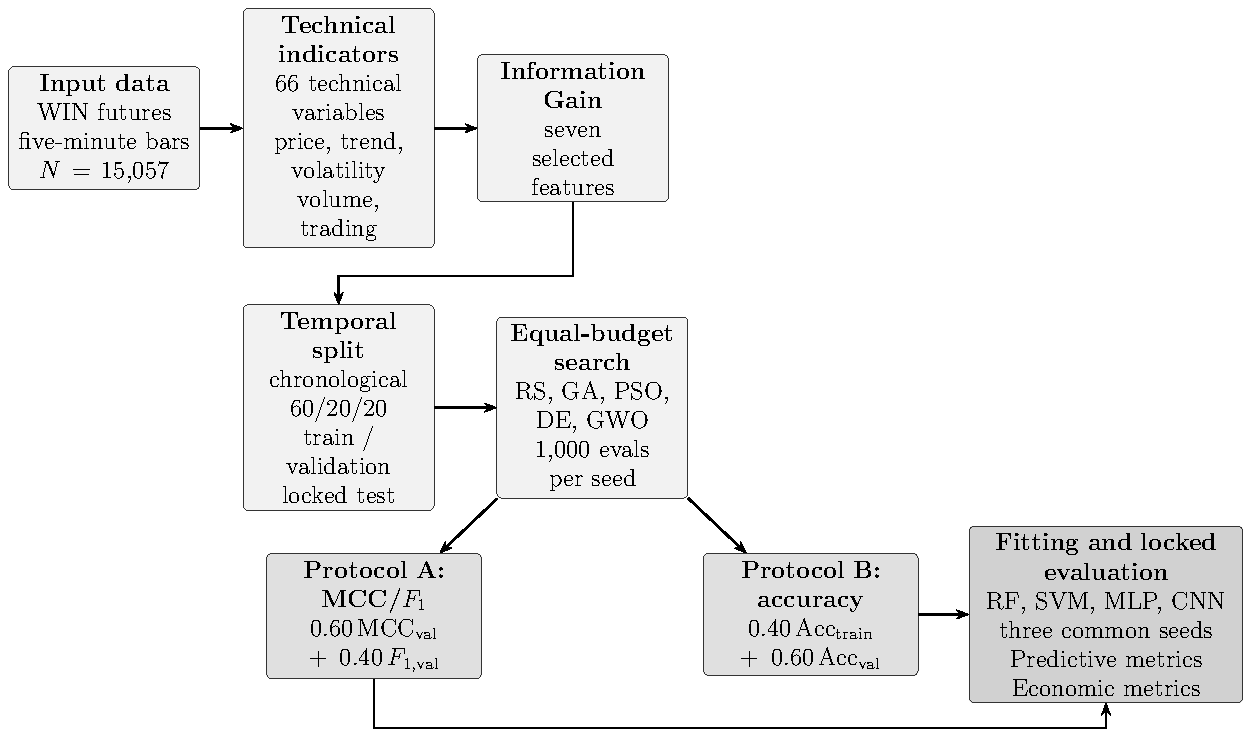
\includegraphics[width=0.96\linewidth]{figures/methodology_workflow_vector.pdf}
\caption{Overview of the proposed methodology. The benchmark reuses the precursor's fixed Information-Gain representation while enforcing a chronological split, equal optimizer budget, and two separated validation objectives.}
\label{fig:workflow}
\end{figure}

Table~\ref{tab:experimental_protocol} consolidates the decisions that define the experimental unit. It is included to make clear which conditions are held fixed while optimizers and classifier backbones vary. Detailed search domains and algorithm-specific update settings are provided in the subsequent subsections.

\begin{table}[htbp]
\centering
\caption{Reproducible experimental protocol. All candidates within a model--optimizer--seed cell use the same fixed representation, chronological partition, and evaluation budget.}
\label{tab:experimental_protocol}
\small
\begin{tabularx}{\linewidth}{@{}p{0.31\linewidth} L@{}}\toprule
\textbf{Component} & \textbf{Specification}\\\midrule
Data & 15,057 five-minute WIN records from January--June 2024; next-bar binary direction target.\\
Input representation & Fixed seven-indicator Information-Gain mask inherited from the blinded precursor.\\
Partition & Chronological 60/20/20 split: 9,034 training, 3,011 validation, and 3,012 locked-test observations.\\
Backbones & Random Forest, Support Vector Machine, Multilayer Perceptron, and 1D Convolutional Neural Network.\\
Search methods & Random Search, Genetic Algorithm, Particle Swarm Optimization, Differential Evolution, and Grey Wolf Optimizer.\\
Budget and repetition & 1,000 candidate evaluations per optimizer, model, and seed; common seeds 1--3. Population methods use 10 candidates for 100 iterations.\\
Selection objectives & Protocol A: $0.60\,\mathrm{MCC}_{\mathrm{val}}+0.40\,F_{1,\mathrm{val}}$; Protocol B: $0.40\,\mathrm{Acc}_{\mathrm{train}}+0.60\,\mathrm{Acc}_{\mathrm{val}}$.\\
Preprocessing and refit & Standardizer fitted on training only during search; final selected configuration refitted on training plus validation before one locked-test evaluation.\\
Reported endpoints & Locked-test accuracy, MCC, $F_1$, exploratory model-level inference, and fixed-rule intrabar economic outcomes.\\\bottomrule
\end{tabularx}
\end{table}

\subsection{Input Data}
\label{sec:data}

The data were obtained from the BovDB resources \cite{cardoso2022bovdb}. The analyzed subset contains 15,057 clean five-minute records of the WIN contract from January to June 2024. WIN is referenced to the Ibovespa index and was selected because its liquidity and frequent intraday movement make it suitable for short-horizon computational prediction. The binary target indicates the next-bar direction: 0 for downtrend and 1 for uptrend.

The records remain in chronological order. The first 9,034 observations are used for training, the subsequent 3,011 observations for validation, and the final 3,012 observations for locked testing. No random shuffling is applied. Figure~\ref{fig:partition} makes this separation explicit; the test observations are unavailable during hyperparameter selection and final model choice.

\begin{figure}[htbp]
\centering
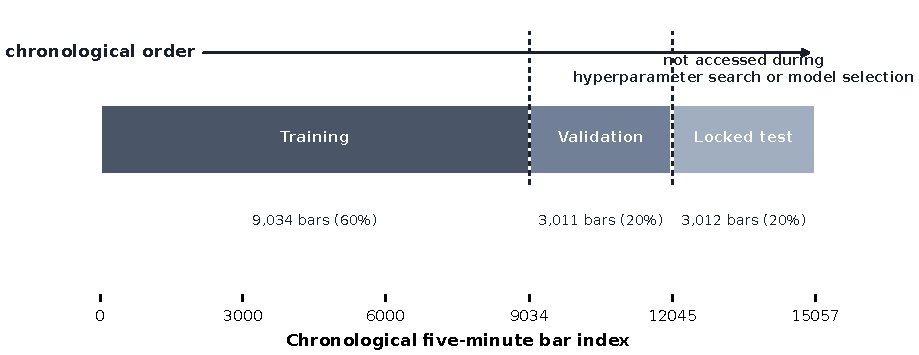
\includegraphics[width=0.93\linewidth]{figures/ijcnn_style_partition.pdf}
\caption{Chronological data partition used in every experiment. Training, validation, and locked test segments occupy consecutive periods of the WIN five-minute series.}
\label{fig:partition}
\end{figure}

\subsection{Generation of Technical Analysis Indicators}
\label{sec:indicators}

Technical indicators were derived from open, high, low, close, trade volume, and transaction-frequency information. Simple Moving Average (SMA), Exponential Moving Average (EMA), and dispersion measures were computed over short windows (3, 5, 7, and 9 periods) to retain sensitivity to intraday changes. For example, the difference between the seven- and three-period SMA is
\begin{equation}
\mathrm{SMA}_{7-3}=\mathrm{SMA}_{7}-\mathrm{SMA}_{3}.
\end{equation}
Together, the construction procedure produces 66 descriptors, including moving-average differences and normalized counterparts. For each optimizer evaluation, feature standardization is fitted on the training partition only and then applied unchanged to the validation partition. For the final locked-test evaluation, a new standardization transform is fitted on the combined training--validation block and applied to the test block only.

\subsection{Feature Selection Method}
\label{sec:featureselection}

The current benchmark reuses a fixed seven-variable mask obtained by Information Gain in the blinded precursor rather than re-estimating the filter in each current split \cite{anonymous2026precursor}. The fixed mask contains EMA$_{5-3}$, normalized EMA$_{5-3}$, EMA$_{7-3}$, normalized EMA$_{7-3}$, normalized SMA$_9$, EMA$_{9-3}$, and normalized EMA$_7$. It is therefore applied identically to every backbone, optimizer, and seed, isolating the optimizer comparison from changes in input representation. This choice does not independently revalidate the feature-selection stage on the present training segment; the reported evidence concerns hyperparameter search conditional on this inherited representation.

\subsection{Implemented Classifier Architectures and Search Spaces}
\label{sec:classifier_architectures}

To benchmark metaheuristic search performance across fundamentally distinct hypothesis spaces, four classifier backbones were implemented: Random Forest (RF), Support Vector Machines (SVM), Multilayer Perceptron (MLP), and 1D Convolutional Neural Networks (1D-CNN). Figure~\ref{fig:classifier_backbones} illustrates the structural decision mechanisms and layer topologies of these four implemented architectures.

\begin{figure}[htbp]
\centering
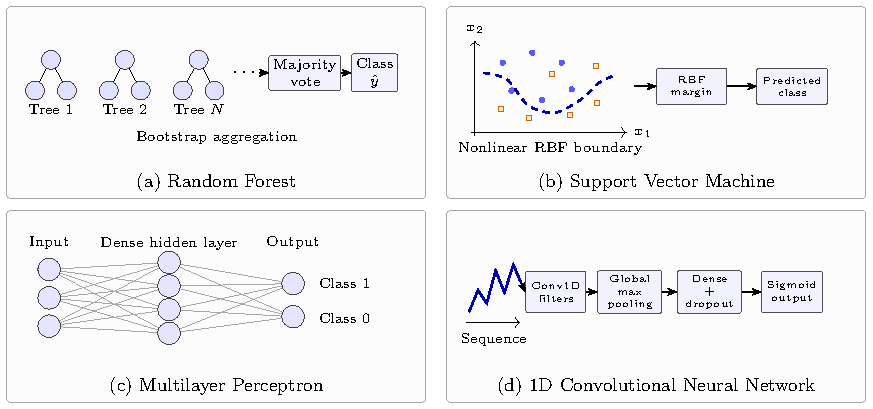
\includegraphics[width=\linewidth]{figures/classifier_backbones_vector.pdf}
\caption{Simplified vector schematics of the four classifier backbones evaluated under the equal-budget metaheuristic optimization framework: (a) Random Forest, (b) Support Vector Machine, (c) Multilayer Perceptron, and (d) 1D Convolutional Neural Network.}
\label{fig:classifier_backbones}
\end{figure}

The hyperparameter search space bounds $\bm{\theta} \in \mathcal{S}$ for each implemented model are defined as follows:
\begin{itemize}
    \item \textbf{RF}: Number of trees $n_{\text{estimators}} \in [50,500]$, maximum tree depth $d_{\text{max}} \in [5,50]$, minimum split samples $s_{\text{split}} \in [2,20]$, minimum leaf samples $s_{\text{leaf}} \in [1,20]$, and categorical choices for \texttt{max\_features} ($\{\texttt{sqrt},\texttt{log2},\texttt{None}\}$) and \texttt{class\_weight} ($\{\texttt{None},\texttt{balanced}\}$).
    \item \textbf{SVM}: Soft-margin penalty $C \in [10^{-3},10^3]$ and kernel bandwidth $\gamma \in [10^{-5},10^1]$, both sampled on logarithmic scales, with linear and radial-basis-function kernels considered.
    \item \textbf{MLP}: Hidden-layer width $n_{\text{hidden}} \in [5,500]$, L2 penalty coefficient $\alpha \in [10^{-8},10^{-2}]$, initial learning rate $\eta_0 \in [10^{-8},10^{-2}]$, dropout $p_{\text{drop}} \in [0,0.10]$, and batch size in $\{16,32,64,80,112,128\}$.
    \item \textbf{1D-CNN}: Filter count $n_{\text{filter}} \in [8,128]$, kernel size $k_{\text{size}} \in [2,5]$, dense-layer width $n_{\text{dense}} \in [16,256]$, L2 penalty coefficient $\alpha \in [10^{-8},10^{-2}]$, Adam learning rate $\eta \in [10^{-8},10^{-2}]$, dropout $p_{\text{drop}} \in [0,0.10]$, and batch size in $\{16,32,64,80,112,128\}$.
\end{itemize}

\subsection{Optimizer Configuration, Search Operators, and Validation Objectives}
\label{sec:optimizerconfiguration}

To ensure complete experimental reproducibility, five search paradigms were evaluated: Random Search (RS), Genetic Algorithm (GA), Particle Swarm Optimization (PSO), Differential Evolution (DE), and Grey Wolf Optimizer (GWO). All optimizers operate under a strict candidate evaluation cap of $N_{\mathrm{eval}} = 1{,}000$ per model and random seed. For all population-based algorithms (GA, PSO, DE, GWO), the population size is fixed to $N_{\mathrm{pop}} = 10$ candidates evaluated across $G = 100$ generations or iterations ($10 \times 100 = 1{,}000$ function evaluations). RS generates $N_{\mathrm{eval}} = 1{,}000$ independent uniform random samples across the search space.

Candidate vectors use the bounds stated above. Integer parameters and categorical-option indices are rounded and clipped to their admissible bounds:
\begin{equation}\label{eq:decoding_discrete}
\theta_d = \mathrm{clip}\!\left(\mathrm{round}(u_d),\theta_{d,\mathrm{min}},\theta_{d,\mathrm{max}}\right).
\end{equation}
For continuous parameters defined on logarithmic scales (such as $C$, $\alpha$, and learning rates), optimizers act on $u_d\in[\log_{10}(\theta_{d,\mathrm{min}}),\log_{10}(\theta_{d,\mathrm{max}})]$ and values are decoded by
\begin{equation}\label{eq:decoding_log}
\theta_d = 10^{u_d}.
\end{equation}

The specific search operators and update formulations governing each optimizer are defined as follows:
\begin{itemize}
    \item \textbf{Genetic Algorithm (GA)}: Utilizes tournament selection ($k=3$), uniform crossover with probability $P_c = 0.80$, and mutation with probability $P_m = 0.20$. When a gene is mutated, its perturbation scale is 0.10 of the corresponding encoded search range.
    \item \textbf{Particle Swarm Optimization (PSO)}: Velocity vectors $\mathbf{v}_i$ and positions $\mathbf{u}_i$ for particle $i$ at iteration $g$ are updated using inertia weight $w = 0.70$ and cognitive/social coefficients $c_1 = c_2 = 1.50$:
    \begin{equation}\label{eq:pso_update}
    \mathbf{v}_i^{g+1} = w \mathbf{v}_i^g + c_1 r_1 (\mathbf{pbest}_i - \mathbf{u}_i^g) + c_2 r_2 (\mathbf{gbest} - \mathbf{u}_i^g),
    \end{equation}
    \begin{equation}
    \mathbf{u}_i^{g+1} = \mathrm{clip}\left(\mathbf{u}_i^g + \mathbf{v}_i^{g+1}, 0, 1\right),
    \end{equation}
    where $r_1, r_2 \sim U(0, 1)$.
    \item \textbf{Differential Evolution (DE)}: Implements the DE/best/1/bin strategy with mutation factor $F = 0.80$ and binomial crossover probability $CR = 0.90$:
    \begin{equation}\label{eq:de_update}
    \mathbf{v}_i^{g+1} = \mathbf{gbest}^g + F (\mathbf{u}_{r1}^g - \mathbf{u}_{r2}^g),
    \end{equation}
    where $r1, r2$ are distinct randomly chosen population indices.
    \item \textbf{Grey Wolf Optimizer (GWO)}: Candidate position vectors are updated by simulating encirclement of the three leading wolves ($\bm{\alpha}, \bm{\beta}, \bm{\delta}$):
    \begin{equation}\label{eq:gwo_update}
    \mathbf{u}_i^{g+1} = \frac{\mathbf{x}_1 + \mathbf{x}_2 + \mathbf{x}_3}{3},
    \end{equation}
    where $\mathbf{x}_1 = \bm{\alpha} - \mathbf{A}_1 \cdot |\mathbf{C}_1 \cdot \bm{\alpha} - \mathbf{u}_i^g|$, with analogous terms for $\mathbf{x}_2$ ($\bm{\beta}$) and $\mathbf{x}_3$ ($\bm{\delta}$).
\end{itemize}

Candidate configurations are evaluated against two separated validation objectives:
\begin{itemize}
    \item \textbf{Protocol A (MCC/$F_1$ Compound Objective)}:
    \begin{equation}\label{eq:fitness_protocol_a}
    f_{\mathrm{MCC/F1}}(\boldsymbol{\theta}) = 0.60\,\mathrm{MCC}_{\mathrm{val}}(\boldsymbol{\theta}) + 0.40\,F_{1,\mathrm{val}}(\boldsymbol{\theta}).
    \end{equation}
    \item \textbf{Protocol B (Weighted Accuracy Objective)}:
    \begin{equation}\label{eq:fitness_protocol_b}
    f_{\mathrm{Acc}}(\boldsymbol{\theta}) = 0.40\,\mathrm{Accuracy}_{\mathrm{train}}(\boldsymbol{\theta}) + 0.60\,\mathrm{Accuracy}_{\mathrm{val}}(\boldsymbol{\theta}).
    \end{equation}
\end{itemize}

Upon completion of the $N_{\mathrm{eval}} = 1{,}000$ search budget, the optimal candidate vector $\boldsymbol{\theta}^* = \arg\max f(\boldsymbol{\theta})$ is refit on the concatenated training and validation dataset ($N = 12{,}045$ bars) and evaluated exactly once on the locked test block ($N = 3{,}012$ bars). The exploratory economic assessment maps an uptrend prediction to a long position and a downtrend prediction to a short position, opened at the bar open and closed at its close. Each bar is treated as one round-trip trade and is charged a fixed cost of five index points. We report total net profit, maximum drawdown, profit factor, and annualized Sharpe ratio; these quantities are therefore specific to this simplified intrabar execution rule rather than a claim of deployable live performance.

\subsection{Statistical Analysis}
\label{sec:statistical_analysis}

Statistical comparisons are conducted separately within each holdout protocol and use the four classifier backbones as the groups of interest. For a given endpoint, each optimizer--seed pair defines one matched block, giving 15 blocks (five optimizers and three seeds) per protocol. We first apply the Friedman rank test to assess whether model outcomes differ across these matched blocks. When summarizing pairwise contrasts, the model with the highest marginal mean for the endpoint is compared with each of the other three models using two-sided paired Wilcoxon signed-rank tests. The resulting three $p$-values are adjusted together using the Holm step-down procedure, with family-wise significance level $\alpha=0.05$.

These tests are exploratory. The blocks share one chronological test segment, and the five optimizers and three seeds do not provide 15 independent market periods. Accordingly, the tests quantify consistency of model ordering across the evaluated optimizer--seed combinations on this fixed test period; they do not establish replication across market regimes or a confirmatory difference between validation protocols. No optimizer-superiority claim is inferred from these model-level tests.
